\chapter{Data structure description language}\label{sec:dsdl}

The data structure description language (DSDL) is used to define data structures for exchange via the CAN bus.
DSDL definitions are used to automatically (or manually) generate the message or service
serialization/deserialization code in a particular programming language.
A tool that automatically generates source code from DSDL definition files is called a \emph{DSDL compiler}.

\section{File hierarchy}

Each DSDL definition file specifies exactly one data structure that can be used for message broadcasting,
or a pair of structures that can be used for service invocation (request and response).

A DSDL source file is named using the \emph{short data type name},
the semantic version number pair (major and minor; see the section \ref{sec:dsdl_versioning}
for more information on data type versioning),
and the \emph{default data type ID} (if needed) as shown
below\footnote{In this declaration, the mandatory parts are surrounded with angle brackets,
and the optional parts are surrounded with square brackets.}:

\verb|[default DTID.]<short name>.<major version number>.<minor version number>.uavcan|

Every defined data structure is contained in a namespace,
which may in turn be \emph{nested} within another namespace.
A namespace that is not nested in another namespace is called a \emph{root namespace}.
For example, all standard data types are contained in the root namespace \verb|uavcan|,
which contains nested namespaces, such as \verb|protocol|.

The namespace hierarchy is mapped directly to the file system directory structure,
as shown in the example below:

\begin{minted}[linenos=false]{text}
uavcan/                           <- Root namespace
    equipment/                    <- Nested namespace
        ...
    protocol/                     <- Nested namespace
        341.NodeStatus.1.0.uavcan <- Data type "uavcan.protocol.NodeStatus" v1.0 with default DTID 341
        ...
    Timestamp.uavcan              <- Data type "uavcan.Timestamp", default DTID is not assigned
\end{minted}

Notes:

\begin{itemize}
    \item It is not necessary to explicitly define a default data type ID for non-standard data types
          (i.e., for vendor-specific or application-specific data types).
    \begin{itemize}
        \item If the default data type ID is not defined by the DSDL definition,
              it will need to be assigned by the application at run time.
        \item All standard data types have default data type ID values defined.
    \end{itemize}

    \item Data type names are case sensitive, i.e., names \verb|foo.Bar| and \verb|foo.bar| are considered different.
          Names that differ only in case should be avoided, because it may cause problems on file systems that are not
          case-sensitive.

    \item Data types may contain nested data structures.
    \begin{itemize}
        \item Some data structures may be designed for such nesting only,
              in which case they are not required to have a dedicated data type ID at all
              (neither default nor runtime-assigned).
    \end{itemize}

    \item \emph{Full data type name} is a unique identifier of a data type constructed from the root namespace,
          all nested namespaces (if any), and the short data type name, joined via the dot symbol (\verb|.|),
          e.g., \verb|uavcan.protocol.file.Read|.
    \begin{itemize}
        \item The total length of the full data type name must not exceed 80 characters.
        \item Refer to the naming rules below for the limitations imposed on the character set.
    \end{itemize}
\end{itemize}

\subsection{Service data types}

Since a service invocation consists of two independent network data exchange operations,
the DSDL definition for a service must define two structures:

\begin{description}
    \item[Request part] - for the request transfer (client to server).
    \item[Response part] - for the response transfer (server to client).
\end{description}

Both request and response structures are contained within the same DSDL definition file,
separated by a special statement as defined in the section \ref{sec:dsdl_syntax}.

Service invocation data structures cannot be nested into other structures.

\section{Syntax}\label{sec:dsdl_syntax}

A data structure definition is a collection of statements.
Each statement is located on a separate line.
Lines are separated with the ASCII line feed character (\verb|\n|, code 10),
or with a sequence consisting of the ASCII carriage return character followed by the ASCII line feed character
(\verb|\r\n|, code 13 and 10, respectively).

The following types of statements are defined:

\begin{description}
    \item[Attribute] - used to define entities of the data type, such as data fields and constants.
    \item[Directive] - directives provide instructions to the DSDL compiler.
    \item[Service response marker] - separates the request and response parts of a service data type definition.
\end{description}

An attribute can be either of the following:

\begin{description}
    \item[Field] - a variable that can be modified by the application and exchanged via the network.
    \item[Constant] - an immutable value that does not participate in network exchange.
\end{description}

DSDL source files may also contain human-readable comments, which are ignored by the compiler.

A message data type definition may contain the following entities:

\begin{itemize}
    \item Attribute definitions
    \item Directives
    \item Comments
\end{itemize}

A service data type definition may contain the following entities:

\begin{itemize}
    \item Request part attribute definitions
    \item Response part attribute definitions
    \item Request part directives
    \item Response part directives
    \item Comments
    \item Service response marker (always exactly one marker) (section \ref{sec:dsdl_service_response_marker})
\end{itemize}

Unless specifically stated otherwise,
directives apply only to the part of the service type definition where they are defined,
not crossing the boundary of the service response marker.

\subsection{Attribute definition}

Field definitions follow one of the below specified declaration patterns:

\begin{itemize}
    \item \verb|cast_mode field_type field_name|
    \item \verb|cast_mode field_type[X] field_name|
    \item \verb|cast_mode field_type[<X] field_name|
    \item \verb|cast_mode field_type[<=X] field_name|
    \item \verb|void_type|
\end{itemize}

Constant definitions are formed using the following declaration patterns:

\begin{itemize}
    \item \verb|cast_mode constant_type constant_name = constant_initializer|
\end{itemize}

Each component of the specified patterns is reviewed in detail below.

\subsubsection{Field type}

A field type declaration can be either a primitive data type
(primitive data types are defined in section \ref{sec:dsdl_primitive_data_types}) or a nested data structure.

A primitive data type is referred simply by its name, e.g., \verb|float16|, \verb|bool|.

A nested data structure is referred by its name and the version number,
separated by the ASCII dot (full stop) character.
The name can be either the full name or the short name.
The latter option is permitted only if the referred data type is located in the same namespace as
the referring data type.
The version number can be either the major version number, or both the major and the minor version
numbers separated by the ASCII dot (full stop) character.
In the former case, the highest available minor version number is implied.
Consider the following examples,
where all of the declarations refer to the same nested data type, assuming that the referring definition is
located in the namespace \verb|uavcan.protocol|:

\begin{minted}[linenos=false]{text}
NodeStatus.1
NodeStatus.1.0
uavcan.protocol.NodeStatus.1
uavcan.protocol.NodeStatus.1.0
\end{minted}

A field type name can be appended with a statement in square brackets to define an array:

\begin{itemize}
    \item Syntax \verb|[X]| is used to define a static array of size exactly X items.
    \item Syntax \verb|[<X]| is used to define a dynamic array of size from 0 to X-1 items, inclusively.
    \item Syntax \verb|[<=X]| is used to define a dynamic array of size from 0 to X items, inclusively.
\end{itemize}

In the array definition statements above, \verb|X| must be a valid
integer literal according to the rules defined in the section \ref{sec:dsdl_constant_definition}.

Observe that the maximum size of dynamic arrays is always bounded,
this ensures that the worst case memory footprint and associated computational complexity are predictable.

\subsubsection{Field name and constant name}

For a message data type, all attributes must have a unique name within the data type definition.

For a service data type, all attributes must have a unique name within the same part (request/response) of
the data type definition.
In other words, service type attributes can have the same name as long as they are separated by
the service response marker (section \ref{sec:dsdl_service_response_marker}).

Restrictions on the character set and further information are provided in the section \ref{sec:dsdl_naming_rules}.

\subsubsection{Cast mode}

Cast mode defines the rules of conversion from native values of a particular programming language
to serialized field values.
Cast mode may be left undefined, in which case the default will be used.
Cast mode cannot be specified for nested data structures and void field types.
The possible cast modes are defined below.

\begin{itemize}
    \item \verb|saturated| - this is the default cast mode,
          which will be used if the attribute definition does not specify the cast mode explicitly.
          For integers, it prevents an integer overflow, replacing it with saturation -
          for example, an attempt to write 0x44 to a 4-bit field
          will result in a bit field value of 0x0F.
          For floating point values, it prevents overflow when casting to a lower precision floating point
          representation - for example, 65536.0 will be converted to a \verb|float16| as 65504.0;
          infinity will be preserved.
    \item \verb|truncated| - for integers, discards the excessive most significant bits;
          for example, an attempt to write 0x44 to a 4-bit field will produce 0x04.
          For floating point values, overflow during downcasting will produce an infinity.
\end{itemize}

\subsubsection{Constant definition}\label{sec:dsdl_constant_definition}

A constant must be of a primitive (section \ref{sec:dsdl_primitive_data_types}) scalar type.
Arrays and nested data structures are not allowed as constant types.

A constant must be assigned with a constant initializer, which must be one of the following:

\begin{itemize}
    \item Integer zero (0).
    \item Integer literal in base 10, starting with a non-zero character. E.g., \verb|123|, \verb|-12|.
    \item Integer literal in base 16 prefixed with \verb|0x|. E.g., \verb|0x123|, \verb|-0x12|, \verb|+0x123|.
    \item Integer literal in base 2 prefixed with \verb|0b|. E.g., \verb|0b1101|, \verb|-0b101101|, \verb|+0b101101|.
    \item Integer literal in base 8 prefixed with \verb|0o|. E.g., \verb|0o123|, \verb|-0o777|, \verb|+0o777|.
    \item Floating point literal. Fractional part with an optional exponent part,
          e.g., \verb|15.75|, \verb|1.575E1|, \verb|1575e-2|, \verb|-2.5e-3|, \verb|+25E-4|.
          Not-a-number (NaN), positive infinity, and negative infinity are intentionally not supported
          in order to maximize cross-platform compatibility.
    \item Boolean \verb|true| or \verb|false|.
    \item Single ASCII character, ASCII escape sequence, or ASCII hex literal in single quotes. E.g.,
          \verb|'a'|, \verb|'\x61'|, \verb|'\n'|.
\end{itemize}

The DSDL compiler must convert the initializer expression to its constant type
if the target type can allocate the value with no data loss.
If a data loss occurs (e.g., integer overflow, floating point number decays to infinity, etc.),
the DSDL compiler must refuse to compile such data type.

Note that constants do not affect the serialized data layout as they are never exchanged via the network.

\subsubsection{Void type}

Void type is a special field type that is intended for data alignment purposes.
The specification defines 64 distinct void types as follows:

\begin{itemize}
    \item \verb|void1| - 1 padding bit;
    \item \verb|void2| - 2 padding bits;
    \item \ldots
    \item \verb|void63| - 63 padding bits;
    \item \verb|void64| - 64 padding bits.
\end{itemize}

A field of a void type does not have a name and its cast mode cannot be specified.
During message serialization, all void fields are filled with zero bits;
during deserialization, the contents of void fields should be ignored.

\subsection{Directives}\label{sec:dsdl_directives}

A directive is a single case-sensitive word starting with an ASCII "at sign" character (\verb|@|),
possibly followed by space-separated arguments:

\begin{minted}[linenos=false]{text}
@directive
@directive arg1 arg2
\end{minted}

All valid directives are documented in this section.

\subsubsection{Union}

Keyword: \verb|@union|.

This directive instructs the DSDL compiler that the current message or the current part of a service data type
(request or response) is a \emph{tagged union}.
A tagged union is a data structure that may encode any one of its fields at a time.
Such a data structure contains one implicit field - the \emph{union tag} - that indicates which particular
field the data structure is holding at the moment.
Unions are required to have at least two fields.

This directive must be placed before the first attribute definition.

\subsection{Comments}

A DSDL description may contain comments starting from the ASCII number sign (\verb|#|)
up until the end of the current line.
Comments are ignored by DSDL compilers.

\subsection{Service response marker}\label{sec:dsdl_service_response_marker}

A service response marker separates the request and response parts of a service data type definition.
The marker consists of three ASCII minus symbols (\verb|-|) in a row on a dedicated line:

\begin{minted}[linenos=false]{text}
---
\end{minted}

The request part precedes the marker, and the response part follows the marker.
The presence of a service response marker indicates that the current definition is a
service type definition rather than a message type definition.

\section{Primitive data types}\label{sec:dsdl_primitive_data_types}

These types are assumed to be built-in.
They can be directly referenced from any data type of any namespace.
The DSDL compiler should implement these types using the native types of the target programming language.
An example mapping to native types is given here for C/C++.

\begin{UAVCANSimpleTable}{Primitive data types}{|l l l X|}\label{table:dsdl_primitive_data_types}
    Name                    & Bit length    & Possible representation in C/C++  & Value range \\
    \texttt{bool}           & $1$
                            & \texttt{bool} (can be optimized for bit arrays)
                            & $\{0, 1\}$
                            \\
    \texttt{int\textbf{X}}  & $2 \le{} \text{X} \le 64$
                            & \texttt{int8\_t}, \texttt{int16\_t}, \texttt{int32\_t}, \texttt{int64\_t}
                            & $\lbrack -\frac{2^\text{X}}{2}, \frac{2^\text{X}}{2} - 1\rbrack$
                            \\
    \texttt{uint\textbf{X}} & $2 \le{} \text{X} \le 64$
                            & \texttt{uint8\_t}, \texttt{uint16\_t}, \texttt{uint32\_t}, \texttt{uint64\_t}
                            & $\lbrack 0, 2^\text{X} - 1\rbrack$
                            \\
    \texttt{float16}        & $16$
                            & \texttt{float}
                            & $\pm{}65504$
                            \\
    \texttt{float32}        & $32$
                            & \texttt{float}
                            & Approx. $\pm{}10^{39}$
                            \\
    \texttt{float64}        & $64$
                            & \texttt{double}
                            & Approx. $\pm{}10^{308}$
                            \\
    \texttt{void\textbf{X}} & $1 \le{} \text{X} \le 64$
                            & \emph{N/A}
                            & \emph{N/A}
                            \\
\end{UAVCANSimpleTable}

\section{Naming rules}\label{sec:dsdl_naming_rules}

\subsection{Mandatory}

Field names, constant names, and type names must contain only ASCII alphanumeric characters and underscores
\verb|[A-Za-z0-9_]|,
and must begin with an ASCII alphabetic character \verb|[A-Za-z]|.
Violation of this rule must be detected by the DSDL compiler and treated as a fatal error.

\subsection{Optional}

The following rules should be checked by the DSDL compiler, but are not mandatory;
their violation should not be treated as a fatal error:

\begin{itemize}
    \item Field and namespace names should be all-lowercase words separated with underscores,
          and may include numbers, (e.g.: \verb|field_name_123|).

    \item Constant names should be all-uppercase words separated with underscores,
          and may include numbers (e.g.: \verb|CONSTANT_NAME_123|).

    \item Data type names should be in camel case (first letter of each word is uppercase),
          and may include numbers (e.g.: \verb|TypeName123|).
\end{itemize}

\subsection{Advisory}

The following advisory rules should be considered by the data type designer:

\begin{itemize}
    \item Message names should be nouns and/or adjectives (e.g., \verb|BatteryStatus|);
    service names should be imperatives (e.g., \verb|Restart|, \verb|GetNodeInfo|).

    \item The name of a message that carries a command should end with the word "Command";
          the name of a message that carries status information should end with the word "Status".

    \item The name of a service that is designed to obtain or to store data should begin with the word
          "Get" or "Set", respectively.
\end{itemize}

\section{Data serialization}\label{sec:dsdl_data_serialization}

\subsection{General principles}

A serialized data structure of type $A$ is an ordered set of data fields joined together into a bit string
according to the DSDL definition of the data structure $A$.
The ordering of the fields follows that of the data structure definition.

Serialized bit strings do not have any implicit data entities such as padding or headers.
Data type developers are advised\footnote{But not required.} to manually align fields at
byte boundaries using the void data types
in order to simplify data layouts and improve the performance of serialization and deserialization routines.

Serialized fields follow the little-endian byte order\footnote{Least-significant byte (LSB) first.}.
One byte is assumed to contain exactly eight bits.
Bits are filled from the most significant bit to the least significant bit,
i.e., the most significant bit has the index 0.

Serialized data structures must be padded upon completion to one byte,
with the pad bits set to zero.
Lower layers of the protocol may also add additional padding as
necessary\footnote{More on this in the chapter \ref{sec:can_bus_transport_layer}.};
however, the rules and patterns of such padding fall out of the scope of the DSDL specification.

\subsubsection{Example}

Consider the following data type definition:

\begin{minted}{python}
truncated uint12 first
truncated int3   second
truncated int4   third
truncated int2   fourth
truncated uint4  fifth
\end{minted}

It can be seen that the bit layout is rather complicated because the field boundaries do not align with byte
boundaries, which makes it a good case study.
Suppose that we were to encode the above structure with the fields assigned the following values
shown in the comments:

\begin{minted}{python}
truncated uint12 first      # = 0xBEDA (48858)
truncated int3   second     # = -1
truncated int4   third      # = -5
truncated int2   fourth     # = -1
truncated uint4  fifth      # = 0x88 (136)
\end{minted}

The resulting encoded byte sequence is shown on the figure \ref{fig:dsdl_serialization_example}.

\begin{figure}[hbt]
    \centering
	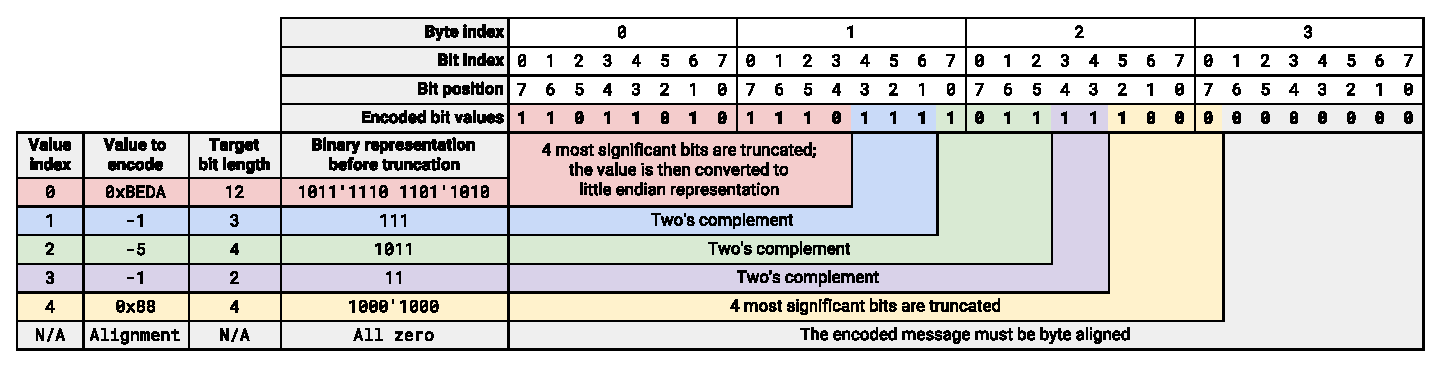
\includegraphics[width=\textwidth]{dsdl/bit-encoding}
	\caption{DSDL serialization example.\label{fig:dsdl_serialization_example}}
\end{figure}

\subsection{Scalar values}

The table \ref{table:dsdl_scalar_serialization} lists the scalar value serialization rules.

\begin{UAVCANSimpleTable}{Scalar value serialization}{|l l X|}\label{table:dsdl_scalar_serialization}
    Type                    & Bit length    & Binary format \\
    \texttt{bool}           & 1
                            & Single bit
                            \\
    \texttt{int\textbf{X}}  & X
                            & Two's complement signed integer
                            \\
    \texttt{uint\textbf{X}} & X
                            & Plain bits
                            \\
    \texttt{float16}        & 16
                            & IEEE 754 binary16
                            \\
    \texttt{float32}        & 32
                            & IEEE 754 binary32
                            \\
    \texttt{float64}        & 64
                            & IEEE 754 binary64
                            \\
    \texttt{void\textbf{X}} & X
                            & X zero bits; ignore when decoding
                            \\
\end{UAVCANSimpleTable}

\subsection{Nested data structures}

Nested data structures are serialized directly in-place,
as if their DSDL definition was pasted directly in place of their reference.
No additional prefixes, suffixes, or padding is provided.

\subsection{Fixed size arrays}

Fixed-size arrays are encoded as a plain sequence of items,
with each item encoded independently in place, with no alignment.
No extra data is added.

Essentially, a fixed-size array of size $X$ elements will be encoded exactly in the same way
as a sequence of $X$ fields of the same type in a row.
Hence, the following two data type definitions will have identical binary representation,
the only actual difference being their representation for the application
if automatic code generation is used.

\begin{minted}{python}
AnyType[3] array
\end{minted}

\begin{minted}{python}
AnyType item_0
AnyType item_1
AnyType item_2
\end{minted}

\subsection{Dynamic arrays}

The following two array definitions are equivalent;
the difference is their representation in the DSDL definition for better readability:
\begin{minted}{python}
AnyType[<42] a      # Can contain from 0 to 41 elements
AnyType[<=41] b     # Can contain from 0 to 41 elements
\end{minted}

A dynamic array is encoded as a sequence of encoded items prepended with an unsigned
integer field representing the number of contained items - the \emph{length field}.
The bit width of the length field is a function of the maximum number of items in the array:
$$\lceil{}\log_2 (X + 1)\rceil{}$$
where $X$ is the maximum number of items in the array.
For example, if the maximum number of items is 251, the length field bit width must be 8 bits;
if the maximum number of items is 1, the length field bit width will be just a single bit.

It is recommended to manually align dynamic arrays by prepending them with void fields
so that the first element is byte-aligned, as that enables more efficient serialization and
deserialization.
This recommendation does not need to be followed if the size of the array elements is not
a multiple of eight bits or if the array elements are of variable size themselves
(e.g., a dynamic array of nested types which contain dynamic arrays themselves).

Consider the following definition:

\begin{minted}{python}
void2                       # Padding - not required, provided as an example
AnyType[<42] array          # The length field is 6 bits wide (see the formula)
\end{minted}

If the array contained three elements,
the resulting binary representation would be equivalent to that of the following definition:

\begin{minted}{python}
void2                       # Padding - not required, provided as an example
uint6 array_length          # Set to 3, because the array contains three elements
AnyType item_0
AnyType item_1
AnyType item_2
\end{minted}

\subsection{Unions}

Similar to dynamic arrays, tagged unions are encoded as two subsequent entities:
the union tag followed by the selected field, with no additional data.

The union tag is an unsigned integer, the bit length of which is a function of the number of fields in the union:
$$\lceil{}\log_2 N\rceil{}$$
where N is the number of fields in the union.
The value encoded in the union tag is the index of the selected field.
Field indexes are assigned according to the order in which they are defined in DSDL,
starting from zero;
i.e. the first defined field has the index 0, the second defined field has the index 1, and so on.

Constants are not affected by the union tag.

It is recommended to manually align unions when they are nested into outer data types by
prepending them with void fields so that the elements are byte-aligned,
as that enables more efficient serialization and deserialization.

Consider the following example:

\begin{minted}{python}
@union                  # In this case, the union tag requires 2 bits
uint16  FOO = 42        # A regular constant attribute
uint16  a               # Index 0
uint8   b               # Index 1
float64 c               # Index 2
uint32  BAR = 42        # Another regular constant
\end{minted}

In order to encode the field \verb|b|, which, according to the definition,
has the data type \verb|uint8|, the union tag should be assigned the value 1.
The following structure will have an identical layout:

\begin{minted}{python}
uint2 tag               # Set to 1
uint8 b                 # The actual data
\end{minted}

If the value of \verb|b| was 7, the resulting encoded byte sequence would be (in binary):
$$%
\underbrace{\texttt{01}}_{\text{tag}}%
\overbrace{\texttt{000001 11}}^{\text{field }\texttt{b}}%
\underbrace{\texttt{000000}}_{\text{padding}}%
$$

\section{Data type compatibility and versioning}\label{sec:dsdl_versioning}

\subsection{Rationale}

As can be seen from the preceding sections,
the concept of \emph{data type} is a cornerstone feature of UAVCAN,
which sets it apart from many competing solutions.

In order to be able to interoperate successfully,
all nodes connected to the same bus must use compatible definitions of all employed data types.
This section is dedicated to the concepts of \emph{data type compatibility}
and \emph{data type versioning}.

A \emph{data type} is a named set of data structures defined in DSDL.
As has been explained above, in the case of message data types,
the set consists of just one data structure, whereas in the case of service data types
the set is a pair of request and response data structures.

Data type definitions may evolve over time as they are refined to better address the needs of their applications.
In order to formalize the data type evolution process with respect to the data type compatibility concerns,
UAVCAN introduces two concepts: \emph{bit compatibility} and \emph{semantic compatibility},
which are discussed below.

\subsection{Bit compatibility}

\subsubsection{Definition}

For the purposes of the definition that follows, an \emph{encoded representation of $A$}
is a sequence of data fields joined into a bit string according to the DSDL definition
of the data structure $A$.

A structure definition $A$ is bit-compatible with a structure definition $B$
if any valid encoded representation of $B$ is also a valid encoded representation of $A$.
$A$ and $B$ are said to be \emph{mutually compatible} if the sets of all possible valid encoded representations of
$A$ and $B$ are identical.

\subsubsection{Example}

A \emph{fixed-size data structure} is a structure that does not contain dynamic arrays
or other structures that contain dynamic arrays within themselves.
As such, the bit length of an encoded representation of a fixed-size structure is constant,
regardless of the data contained in the structure.
Conversely, any data structure that is not fixed-size is called a \emph{variable-size data structure}.

It stands to reason that any data structure definition is compatible with itself.
The following two definitions are bit-compatible as well:

\begin{minted}{python}
uint32 a
uint32 b
\end{minted}

\begin{minted}{python}
uint64 c
\end{minted}

It should be observed that bit-compatibility is invariant to the complexity and the level of nesting
of the data structure.
From the above provided definitions follows that two fixed-size data structures are bit-compatible if the
bit lengths of their respective encoded representations are equal.

Consider the following example data type definition; assume that its full data type name is
\verb|demo.Pair|:

\begin{minted}{python}
# demo.Pair
float16 first
float16 second
\end{minted}

Further, let the following be description of the data type \verb|demo.PairVector|:

\begin{minted}{python}
# demo.PairVector
demo.Pair[3] vector
\end{minted}

Then the following two definitions are bit-compatible:

\begin{minted}{python}
demo.PairVector pair_vector
\end{minted}

\begin{minted}{python}
float16 first_0     # pair_vector.vector[0].first
float16 second_0    # pair_vector.vector[0].second
float16 first_1     # pair_vector.vector[1].first
float16 second_1    # pair_vector.vector[1].second
float16 first_2     # pair_vector.vector[2].first
float16 second_2    # pair_vector.vector[2].second
\end{minted}

The latter definition in the example above is a flattened unrolled form of the former definition.
As such, in that particular example, both definitions can be used interchangeably;
data serialized using one definition can still be meaningful if deserialized using the other definition.
However, it is also possible to construct bit-compatible definitions that are not interchangeable:

\begin{minted}{python}
float16 a
float32 b
\end{minted}

\begin{minted}{python}
float32 a
float16 b
\end{minted}

Even though the above definitions are bit-compatible, one cannot be substituted with the other.
The problem of functional equivalency is addressed by the concept of semantic compatibility,
explored in the section \ref{sec:dsdl_semantic_compatibility}.

The examples above were focused on fixed-size structures.
In the case of fixed-size structures, if $A$ is compatible with $B$, the reverse is also true.
This does not hold for variable-size structures.
Consider the following example:

\begin{minted}{python}
uint8[<=10] a
\end{minted}

\begin{minted}{python}
void1           # The maximum array length is twice lower, so the length prefix is one bit shorter.
uint16[<=5] a   # The 1-bit void field is needed to ensure identical bit offset of the array.
\end{minted}

For the first definition, it is evident that since it contains one dynamic array with
11 possible length values\footnote{Which are 0, 1, 2, 3, 4, 5, 6, 7, 8, 9, and 10.},
and the array type is a fixed-size
structure\footnote{Built-in types can be considered a special case of fixed-size data structures.},
there are 11 possible bit length values for the first definition.

Likewise, for the second definition, there are 6 possible bit length values.

Since both arrays have the same bit offset from the beginning of the bit string,
and taking into account the fact that the element sizes differ by an integral factor,
the set of valid encoded representations of the second definition is a subset of those of the first definition.
Possible encoded representations are summarized in the table \ref{table:dsdl_variable_size_compat},
where the columns labeled "First definition" and "Second definition" contain the number of elements in the
respective arrays.

\begin{minipage}{0.7\textwidth}
\begin{UAVCANSimpleTable}{Variable-size data type compatibility example}{|lll|}\label{table:dsdl_variable_size_compat}
    Bit length  & First definition  & Second definition \\
    4           & 0                 & 0 \\
    12          & 1                 & \emph{invalid} \\
    20          & 2                 & 1 \\
    28          & 3                 & \emph{invalid} \\
    36          & 4                 & 2 \\
    44          & 5                 & \emph{invalid} \\
    52          & 6                 & 3 \\
    60          & 7                 & \emph{invalid} \\
    68          & 8                 & 4 \\
    76          & 9                 & \emph{invalid} \\
    84          & 10                & 5 \\
\end{UAVCANSimpleTable}
\end{minipage}

The table illustrates the fact that the first definition is compatible with the second definition,
but the reverse is not true.

\subsection{Semantic compatibility}\label{sec:dsdl_semantic_compatibility}

\subsubsection{Definition}

A data structure definition $A$ is semantically compatible with a data structure definition $B$
if an application that correctly uses $A$ exhibits a functionally equivalent behavior to an application
that correctly uses $B$,
and $A$ is bit-compatible with $B$.

Because of the dependency on bit compatibility, the property of semantic compatibility is non-commutative.

\subsubsection{Example}

Despite using different binary layouts, the following two definitions are semantically compatible:

\begin{minted}{python}
uint16 FLAG_A = 1
uint16 FLAG_B = 256
uint16 flags
\end{minted}

\begin{minted}{python}
uint8 FLAG_A = 1
uint8 FLAG_B = 1
uint8 flags_a
uint8 flags_b
\end{minted}

Therefore, the definitions can be used
interchangeably\footnote{It should be noted here that due to different set of fields and constants,
the source code auto-generated from the provided definitions may be not drop-in replaceable,
requiring changes in the application. However, application compatibility is orthogonal to
data type compatibility.}.

\subsection{Data type versioning}

\subsubsection{Versioning principles}

Every data type definition has a pair of version numbers -
a major version number and a minor version number, following the principles of semantic versioning.

For the purposes of the following definitions, a \emph{release} of a data type definition stands for
the disclosure of the data type definition to the intended users or to the public,
or for the commencement of usage of the data type definition in a production system.

In order to ensure a deterministic application behavior and ensure a robust migration path
as data type definitions evolve, UAVCAN requires that all data types that share the same major version number
greater than zero must be mutually semantically compatible with each other.

In order to ensure predictable and repeatable behavior of applications that leverage UAVCAN,
the standard requires that once a data type definition is released, it cannot undergo any modifications to
its attributes or directives anymore.
Essentially, released data type definitions are to be considered immutable excepting
comments and whitespace formatting.

Therefore, substantial modifications of released data types are only possible by releasing
new definitions of the same data type.
If it is desired and possible to keep the same major version number for a new definition of the data type,
the minor version number of the new definition shall be one greater than the newest existing minor version
number before the new definition is introduced.
Otherwise, the major version number shall be incremented by one and the minor version shall be set to zero.

An exception to the above rules applies when the major version number is zero.
Data type definitions bearing the major version number of zero are not subjected to any compatibility requirements.
Released data type definitions with the major version number of zero are permitted to change in arbitrary
ways without any regard for compatibility.
It is recommended, however, to follow the principles of immutability, releasing every subsequent definition
with the minor version number one greater than the newest existing definition.

\subsubsection{Major version release constraints}

The DSDL specification limits the number of coexisting major data type versions
in order to simplify support of the data type versioning system at the transport layer
and simplify the management of legacy data type definitions.
As such, at any given moment, the difference between the highest released major version number
and the lowest released major version number of any given data type must not exceed 3.

For example, the following set of released data type definition versions is valid and permissible:
\{0.1, 0.2, 0.3, 1.0, 1.1, 2.0, 2.1, 2.2, 3.0\},
because the difference between the newest released major version (3) and the oldest released major version (0)
does not exceed 3.
The set of the minor versions is not subjected to any constraints,
and as such, there are no limits on the set of concurrently released minor versions.

Continuing with the above example, if it were necessary to release a newer data type definition
under a new major version of 4, the oldest major version of 0 would have to be removed first.
Otherwise, the maximum major version number difference constraint would be violated.
Observe that the actual number of published major versions is irrelevant;
the constraint only applies to the difference between the highest and the lowest released major versions.
For example, shall the version 2 be deprecated and removed while the versions 0 and 1 were still around,
the requirement to remove the version 0 before publishing the version 4 would still hold.
The resulting set of versions may then look like this:
\{1.0, 1.1, 3.0, 4.0\}.

If the difference between the highest and the lowest available major version numbers exceeds 2,
the DSDL compiler must assume that the oldest available definition is marked with an implicit
\verb|@deprecated| directive (section \ref{sec:dsdl_directives}),
even if it is not explicitly provided in the definition.

If the difference between the highest and the lowest available major version numbers exceeds 3,
the DSDL compiler must refuse to process the data type and abort with an error.

\subsubsection{Data type version selection}

There are two aspects to the problem of data type version selection:
compile-time behavior and runtime behavior.
They are explored in this section.

As far as compile-time data type version selection is concerned,
the DSDL compiler is required to compile every available major data type version separately,
allowing the application to choose any available major version at runtime.
However, there may be more than one minor version available per major version;
the DSDL compiler must resolve this ambiguity by always selecting the newest available minor
version per major version at the time of compilation.

For example, consider the following set of data type definition versions:
\{0.1, 0.2, 0.3, 1.0, 1.1, 2.0, 2.1, 2.2, 3.0\}.
As there are four different major data type versions (0, 1, 2, and 3),
the DSDL compiler will make four independent definitions available for the application.
Following the principle of choosing the newest available minor version,
the resulting set of definitions available at runtime will be as follows:
\{0.3, 1.1, 2.2, 3.0\}.

Seeing as the minor version ambiguity is resolved statically,
this information becomes irrelevant for the protocol at runtime.
While implementations can keep the minor version information for diagnostic purposes,
it is completely unnecessary at the transport layer.
As such, the transport layer (which is specified in the chapter \ref{sec:can_bus_transport_layer})
does not concern itself with the minor data type version information,
whereas the major data type version is attached to every transfer.

The implication is that upon reception of a transfer, the node will use the appropriate
data type definition according to the major data type version information attached to the
transfer; whereas the minor versions used by the emitter and the receiver may mismatch.
The possibility of a minor version mismatch is acceptable because, by definition,
all data type definitions sharing the same major version number are mutually semantically compatible.

When initiating a data exchange (e.g. broadcasting a message or invoking a service),
the node is free to choose the major data type version freely, according to its own application logic.
Nodes that provide services (i.e., servers) must respond to requests using the same major service data type
version that was used in the request.
Again, the minor version number may mismatch, but by the compatibility requirement this is acceptable.

\subsubsection{Versioning example}

Suppose a vendor named \emph{Sirius Cybernetics Corporation} was contracted to design a
cryopod management data bus for a colonial spaceship \emph{Golgafrincham B-Ark}.
Having consulted with applicable specifications and standards, an engineer came up with the following
definition of a cryopod status message type (named \verb|sirius_cyber_corp.golgafrincham_b_ark.cryopod.Status|):

\begin{minted}{python}
# sirius_cyber_corp.golgafrincham_b_ark.cryopod.Status.0.1

float16 internal_temperature    # [kelvin]
float16 coolant_temperature     # [kelvin]

# Status flags in the low byte
uint16 FLAG_COOLING_SYSTEM_A_ACTIVE = 1
uint16 FLAG_COOLING_SYSTEM_B_ACTIVE = 2
# Error flags in the high byte
uint16 FLAG_PSU_MALFUNCTION = 8192
uint16 FLAG_OVERHEATING     = 16384
uint16 FLAG_CRYOBOX_BREACH  = 35768
# Storage for the above defined flags
uint16 flags
\end{minted}

The definition has been deployed to the first prototype for initial lab tests.
Since the definition was experimental, the major version number was set to zero, to signify the
tentative nature of the definition.
Suppose that upon completion of the first trials it was identified that the units must track their power consumption
in real time, for each of the three redundant power supplies independently.
The definition has been amended appropriately.

It is easy to see that the amended definition shown below is neither semantically compatible nor bit-compatible
with the original definition; however, it shares the same major version number of zero, because the backward
compatibility rules do not apply to zero-versioned data types to allow for low-overhead experimentation
before the system is fully deployed and fielded.

\begin{minted}{python}
# sirius_cyber_corp.golgafrincham_b_ark.cryopod.Status.0.2

truncated float16 internal_temperature    # [kelvin]
truncated float16 coolant_temperature     # [kelvin]

saturated float32 power_consumption_0     # Power consumption by the redundant PSU 0 [watt]
saturated float32 power_consumption_1     # likewise for PSU 1
saturated float32 power_consumption_2     # likewise for PSU 2

# Status flags in the low byte
uint16 FLAG_COOLING_SYSTEM_A_ACTIVE = 1
uint16 FLAG_COOLING_SYSTEM_B_ACTIVE = 2
# Error flags in the high byte
uint16 FLAG_PSU_MALFUNCTION = 8192
uint16 FLAG_OVERHEATING     = 16384
uint16 FLAG_CRYOBOX_BREACH  = 35768
# Storage for the above defined flags
uint16 flags
\end{minted}

The last definition was deemed sufficient and deployed to the production system
under the version number of 1.0: \verb|sirius_cyber_corp.golgafrincham_b_ark.cryopod.Status.1.0|.

Having collected empirical data from the fielded systems, the Sirius Cybernetics Corporation has
identified a shortcoming in the v1.0 definition, which was corrected in an updated definition.
Since the updated definition, which is shown below, is mutually semantically
compatible\footnote{The topic of data serialization is explored in detail in the section
\ref{sec:dsdl_data_serialization}.}
with v1.0, the major version number was kept the same and the minor version number was incremented by one:

\begin{minted}{python}
# sirius_cyber_corp.golgafrincham_b_ark.cryopod.Status.1.1

saturated float16 internal_temperature    # [kelvin]
saturated float16 coolant_temperature     # [kelvin]

saturated float32[3] power_consumption    # Power consumption by the PSU

# Status flags
uint8 STATUS_FLAG_COOLING_SYSTEM_A_ACTIVE = 1
uint8 STATUS_FLAG_COOLING_SYSTEM_B_ACTIVE = 2
uint8 status_flags

# Error flags
uint8 ERROR_FLAG_PSU_MALFUNCTION = 5
uint8 ERROR_FLAG_OVERHEATING     = 6
uint8 ERROR_FLAG_CRYOBOX_BREACH  = 7
uint8 error_flags
\end{minted}

Since the definitions v1.0 and v1.1 are mutually semantically compatible,
UAVCAN nodes using either of them can successfully interoperate on the same bus.

Suppose further that at some point a newer version of the cryopod module was released,
with higher precision temperature sensors.
The definition has to be updated accordingly to use \verb|float32| for the temperature fields
instead of \verb|float16|.
Seeing as that change breaks the binary compatibility,
the major version number has to be incremented by one, and the minor version number has to be reset back to zero:

\begin{minted}{python}
# sirius_cyber_corp.golgafrincham_b_ark.cryopod.Status.2.0

float32 internal_temperature    # [kelvin]
float32 coolant_temperature     # [kelvin]

float32[3] power_consumption    # Power consumption by the PSU

# Status flags
uint8 STATUS_FLAG_COOLING_SYSTEM_A_ACTIVE = 1
uint8 STATUS_FLAG_COOLING_SYSTEM_B_ACTIVE = 2
uint8 status_flags

# Error flags
uint8 ERROR_FLAG_PSU_MALFUNCTION = 5
uint8 ERROR_FLAG_OVERHEATING     = 6
uint8 ERROR_FLAG_CRYOBOX_BREACH  = 7
uint8 error_flags
\end{minted}

Now, nodes using v1.0, v1.1, and v2.0 definitions can still coexist on the same network,
but they are not guaranteed to understand each other unless they support all of the used data type definitions.

In practice, nodes that need to maximize their compatibility are likely to employ all existing major versions of
each used data type.
If there are more than one minor versions available, the highest minor version within the major version should
be used, to take advantage of the latest changes in the data type definition.
It is also expected that in certain scenarios some nodes may resort to publishing the same message type
using different major versions concurrently to circumvent compatibility issues (in the
example reviewed here that would be v1.1 and v2.0).

\section{Data type ID}

Whenever a data structure is transferred over the bus, it is accompanied by a non-negative integer
- a \emph{data type ID}.
The data type ID (together with the major version number, which is also exchanged over the bus together with the
data type ID) is used by receiving nodes to determine which data type definition to use
to process the received data structure.
The data type ID value does not affect data type compatibility.

It stands to reason that in order to be able to interoperate successfully,
every node connected to the bus must use identical mapping between data types and their identifiers.

There are two independent sets of data type identifiers:
one for message data types and the other for service data types.
Each has a reserved subset which is used for standard data type definitions,
and a dedicated subset for vendor-specific data type definitions.
More info on the reserved subsets is provided in the chapter \ref{sec:application_layer}.

All UAVCAN nodes must use the same data type ID mapping for the standard data types,
as defined by the default data type ID values provided for each of the standard data types.
Since the standard data type ID mapping is immutable, all standard-compliant nodes can always
use standard data types conflict-free.

Vendor-specific data types, however, do not enjoy the lack of conflict guarantee,
because by virtue of being vendor-specific, such data types cannot use a global
fixed agreed upon mapping like the standard data types do.
As such, whenever vendor-specific data types are used, there is always a risk that
different nodes may map different data types to the same data type ID.

It is the responsibility of the system integrator to ensure that if vendor-specific data types are
used, the data type ID mappings are configured on all nodes identically.
Vendors of UAVCAN equipment must provide the integrator with a way to change the data type ID
of any vendor-specific data type leveraged by the node\footnote{Nodes that fail to provide a way of
altering the data type ID mapping for vendor-specific data types cannot be considered standard-compliant}.

\section{Standard and vendor-specific data types}

\subsection{Standard data type repository}

The DSDL definitions of the standard data types are available in the official DSDL repository,
which is linked from the project homepage at \href{http://uavcan.org}{uavcan.org}.

Information concerning development and maintenance of the standard DSDL definitions is available
in the chapter \ref{sec:introduction}.

\subsection{Vendor-specific data types}

Vendors must define their specific data types in a separate namespace,
which should typically be named to match their company name.
Separation of the vendor's definitions into a dedicated namespace ensures that no name conflicts will occur
in systems that utilize vendor-specific data types from different providers.
Note that, according to the naming requirements, the name of a DSDL namespace must start
with an alphabetic character; therefore, a company whose name starts with a digit will have to resort to
a mangled name, e.g. by moving the digits towards the end of the name,
or by spelling the digits in English (e.g. 42 - \verb|fortytwo|).

Defining vendor-specific data types within the standard namespace (\verb|uavcan.|) is explicitly prohibited.
The standard namespace will always be used only for standard data types.

Generally speaking, it is desirable for "generic" data types to be included into the standard set.
Vendors should strive to design their data types as generic and as independent of their specific use
cases as possible.
The SI system of measurement units should be preferred;
data type definitions that make unnecessary deviations from SI will not be accepted into the standard set.

